\documentclass[11pt,xcolor=svgnames]{beamer}
\usepackage{dsfont,natbib,setspace,changepage,multirow}
\mode<presentation>

% replaces beamer foot with simple page number
\setbeamertemplate{navigation symbols}{}
%\setbeamerfont{frametitle}{series=\bfseries}
\setbeamercolor{frametitle}{fg=Black}

\setbeamertemplate{footline}{
   \raisebox{5pt}{\makebox[\paperwidth]{\hfill\makebox[20pt]{\color{gray}\scriptsize\insertframenumber}}}}

\graphicspath{{/Users/mtaddy/Dropbox/inputs/}}
\usepackage{algorithm}
\usepackage{algorithmic}

% colors
\newcommand{\theme}{\color{Maroon}}
\newcommand{\bk}{\color{black}}
\newcommand{\rd}{\color{DarkRed}}
\newcommand{\fg}{\color{ForestGreen}}
\newcommand{\bl}{\color{blue}}
\newcommand{\gr}{\color{black!50}}
\newcommand{\sg}{\color{DarkSlateGray}}
\newcommand{\nv}{\color{Navy}}
\setbeamercolor{itemize item}{fg=gray}
\newcommand{\sk}{\vspace{.25cm}}

% common math markups
\newcommand{\bs}[1]{\boldsymbol{#1}}
\newcommand{\mc}[1]{\mathcal{#1}}
\newcommand{\mr}[1]{\mathrm{#1}}
\newcommand{\bm}[1]{\mathbf{#1}}
\newcommand{\ds}[1]{\mathds{#1}}
\newcommand{\indep}{\perp\!\!\!\perp}
\def\plus{\texttt{+}}
\def\minus{\texttt{-}}

% spacing and style shorthand
\setstretch{1.1}

\begin{document}

\setcounter{page}{0}
{% \usebackgroundtemplate{\includegraphics[height=\paperheight]{phoenix}}
\begin{frame}[plain]
\begin{center}

{\bf \LARGE \theme }

\vskip .25cm
{\bf \LARGE \theme Empirical Bayesian Forests }

\vskip 1cm
Matt Taddy,  Chicago Booth

\vskip .1cm
with Chun-Sheng Chen, Jun Yu, and Mitch Wyle at eBay


\vfill
{\texttt{faculty.chicagobooth.edu/matt.taddy/research}}

\end{center}
\end{frame} }


\begin{frame}
{What is a Decision Tree?}

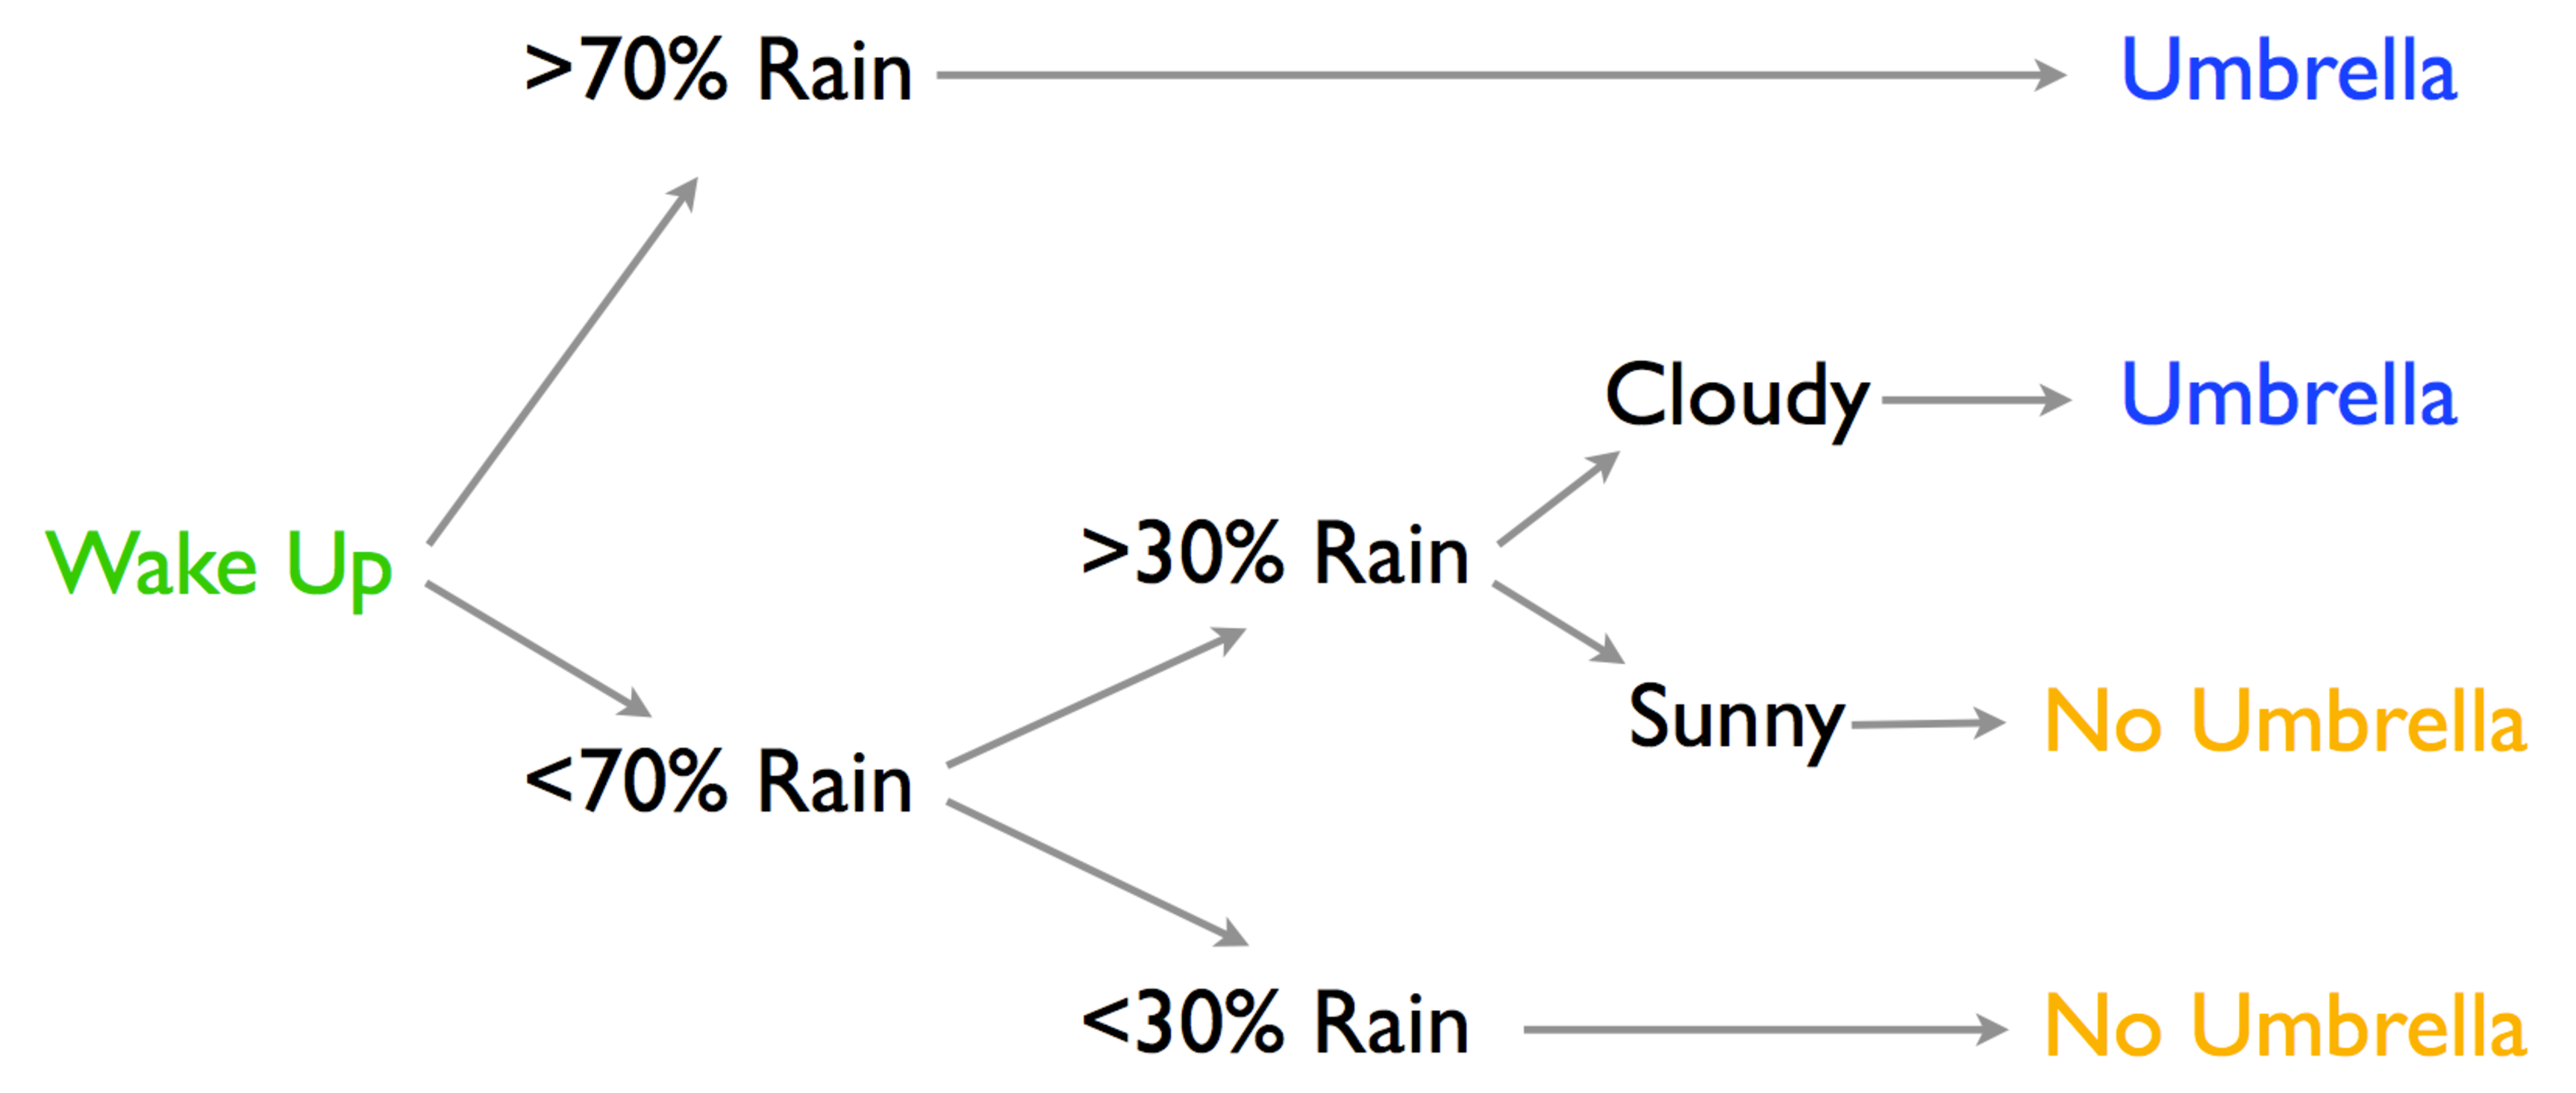
\includegraphics[width=4.25in]{../../bigdata/graphs/umbrella}


\vskip .3cm
\bk Tree-logic uses a series of steps to come to a conclusion.\\
 The trick is to have mini-decisions combine for good choices.
\\ Each decision is a node, and the final prediction is a {\theme
  leaf node}

\end{frame}


\begin{frame}

{\bf Decision Trees are a Regression Model}

\sk
You have inputs $\bm{x}$ {\gr (forecast, current conditions)} \\ and an output of
interest $y$ {\gr (need for an umbrella)}.


\sk 
Based on previous data, the goal is to specify branches of \\ choices 
that lead to good predictions in new scenarios.


{In other words, you want to estimate a {\nv Tree Model}.}


\sk
\bk
Instead of linear coefficients, we need to find `{\theme decision nodes}': \\~~~split-rules defined via thresholds on some dimension of 
$\bm{x}$.

\vskip .5cm
Nodes have a parent-child structure: every node except the root has a parent, and every node except the leaves has two children.


\end{frame}


\begin{frame}

{\bf Decision trees are like a game of mousetrap}

\vskip .25cm
You drop your $\bm{x}$ covariates in at the top, and each decision node
bounces you either left or right.  Finally, you end up in a {\theme leaf node} which contains the data subset defined by these decisions (splits).


\begin{equation*}
\begin{array}{ccccc}
& &  \hskip -2.2cm x_i = 0 &&\\
& & \hskip -2.3cm \swarrow ~~~\searrow &&\\
&  \hskip -.8cm x_j = 2 & & \hskip -2.3cm \{\bm{x}: x_i>0\}&\\
& \hskip -.7cm \swarrow~~~\searrow & & &\\
\{\bm{x}: x_i \leq  0, x_j \leq  2\}& & \hskip -.5cm \{ \bm{x}: x_i \leq 0, x_j>2 \}& &
\end{array}
\end{equation*}

\vskip .5cm
The {\nv prediction rule} at each leaf (a class probability or predicted $\hat y$) is  the average of the sample $y$ values that ended up in that leaf.

\end{frame}


\begin{frame}

Given a {\nv parent} set of data $\{\bm{x}_i,y_i\}_{i=1}^n$, the {\theme optimal split}
is that location $x_{ij}$ on some dimension $j$ on some observation $i$,\\ so that the {\nv child} sets 
\[
\text{\rm{left}:}~\{\bm{x}_k,y_k:~x_{kj} \leq x_{ij}\}
\text{~~and~~\rm{right}:}~\{\bm{x}_k,y_k:~x_{kj} > x_{ij}\}
\]
are as homogeneous in response $y$ as possible.

\vskip .5cm
For example, we will minimize the sum of squared errors \\
\[
\sum_{k \in \mathrm{left}} (y_k - \bar y_{\mathrm{left}})^2 + \sum_{k \in \mathrm{right}} (y_k - \bar y_{\mathrm{right}})^2
\]
for {\it regression trees}, or gini impurity  for {\it classification trees} \\(e.g., the sum across children `c' of $n_{\mathrm{c}}\bar y_{\mathrm{c}}(1-\bar y_{\mathrm{c}})$ if $y\in \{0,1\}$).

\end{frame}

\begin{frame}


{\bf We estimate decision trees by being recursive and greedy}


\vskip .5cm
{\nv CART} grows the tree through a sequence of splits:

\vskip .25cm
\begin{itemize}
\item Given any set (node) of data, you can find the {\theme optimal split} (the error minimizing split) and divide into two child sets.
\item 
We then look at each child set, and again find the optimal split to divide it into two homogeneous subsets.
\item
The children become  parents, and we look again for the optimal split on their new children (the grandchildren!).
\end{itemize}

\vskip .25cm
You stop splitting and growing when the size of the leaf nodes hits some minimum threshold (e.g., say no less than 10 obsv per leaf).

\end{frame}




\begin{frame}


{\bf  Trees are awesome}

\vskip .25cm 
They automatically learn non-linear response functions
\\ and will discover interactions between variables.

\vskip .25cm
Example: Motorcycle Crash Test Dummy Data

\sg
$x$ is time from impact, $y$ is acceleration on the helmet.

\vspace{-1cm}
\begin{adjustwidth}{-.3in}{}
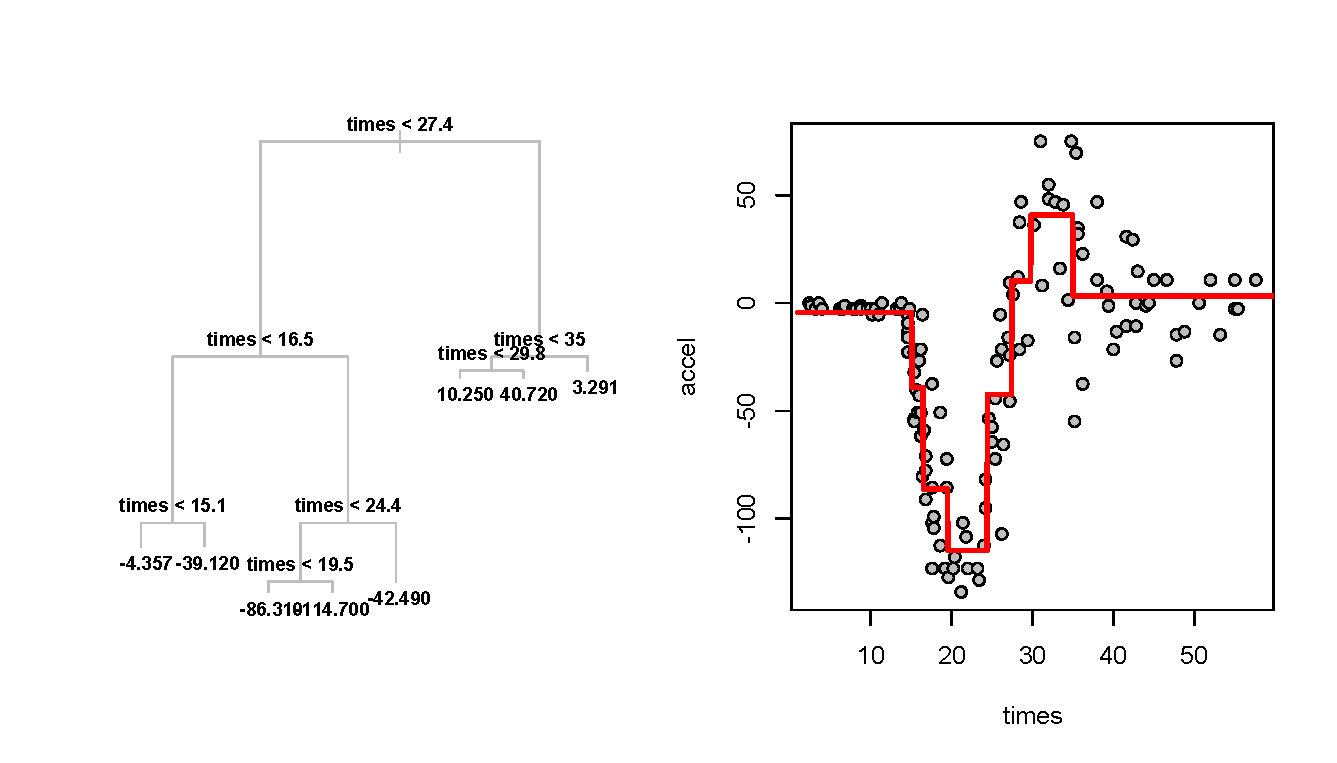
\includegraphics[width=4.6in]{../graphs/MCtree}
\end{adjustwidth}

\vskip -.75cm
\end{frame}


\begin{frame}

{Unfortunately, it is tough to avoid overfit with CART:}

\vskip .1cm \bk
Deep tree structure is so unstable that optimal depth is not easily chosen via cross validation, and there's no theory to fall back on.

\vskip .5cm \bk
Instead, we can average over a {\nv bootstrapped} sample of trees:  

\begin{itemize}
\item repeatedly re-sample the data, {\nv with-replacement}, \\to get a `jittered' dataset of $n$ observations.
\item for each resample, {\nv fit a CART tree}.
\item when you want to predict $y$ for some $\bm{x}$, \\take the {\nv average} prediction from this forest of trees.
\end{itemize}
Real structure that persists across datasets shows up in the average.  Noisy useless signals will average out to have no effect. 

\sk
{\bf \theme \hfill This is a Random Forest {\gr (RF)}}
\end{frame}


\begin{frame}


\begin{center}

\includegraphics[width=.75\textwidth]{../graphs/MCtreedraw}
\end{center}

\vskip -.25cm
Fitting CART to sampled-with-replacement data is equivalent to randomly {\nv weighting} your observations in the deviance calculations. 

\hfill {\gr (size proportional to weight in this picture)}.

\end{frame}

\begin{frame}

{\bf \theme Random Trees \bk for the Motorcycle Data}


\vspace{-1cm}
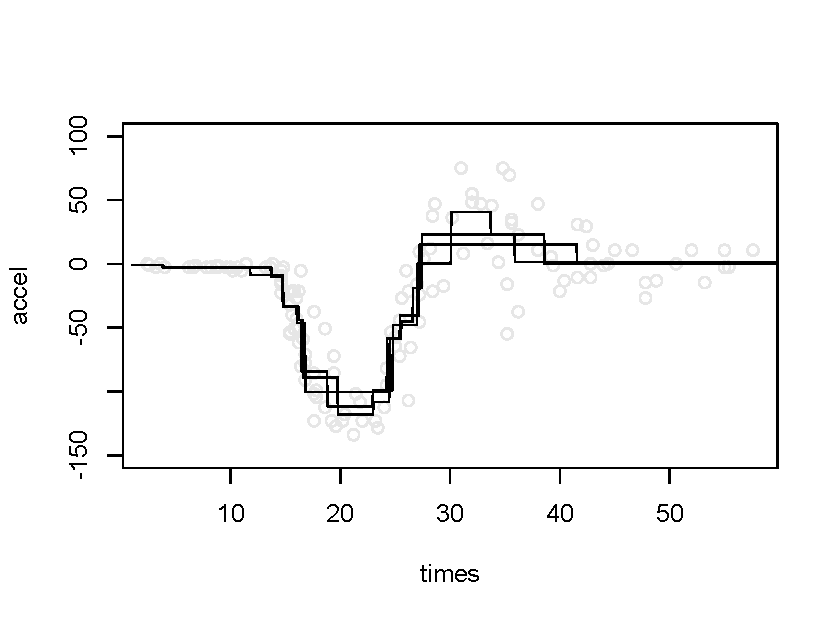
\includegraphics[width=4.25in]{../graphs/MCparticles}

\vskip -.25cm\sg
If you fit to random subsets of the data, \\\nv \hfill you get a slightly different
tree each time.
\vskip -.25cm
\end{frame}


\begin{frame}

{\bf  Model Averaging with \theme Random Forests}

\vskip .25cm
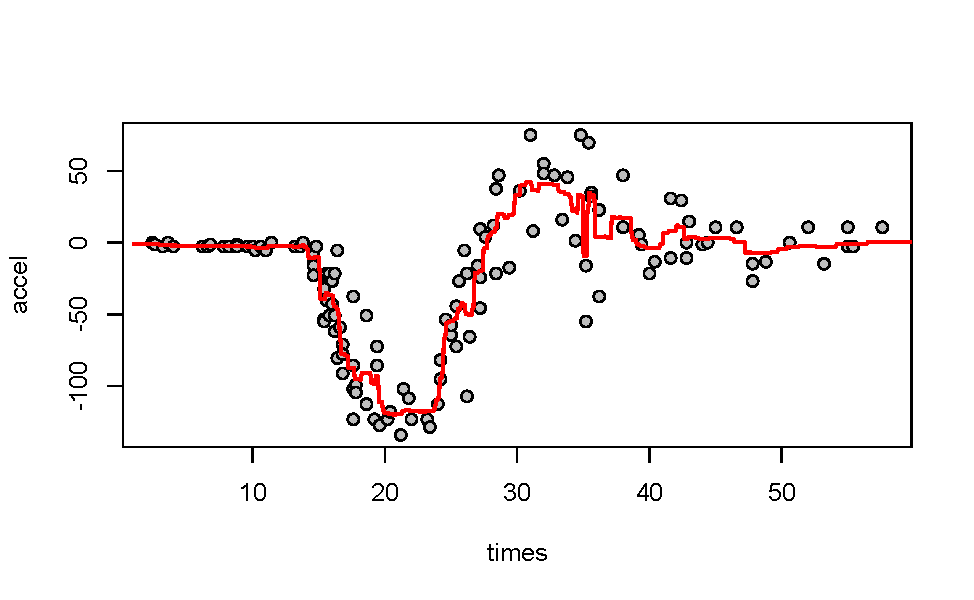
\includegraphics[width=4.35in]{../graphs/MCrf}

\vskip .2cm\sg
Averaging many trees yields a single
[high quality] response surface. 

\vskip -.2cm

\end{frame}

\begin{frame}

{\bf Random Forests are really awesome}

\vskip .25cm
They have all the nice properties of trees, 
while avoiding overfit.

\vskip .25cm
Unfortunately, search for {\it optimal splits} is expensive on Big  data.  

And if one tree is costly, then  many is infeasible (you want many!).

\vskip .75cm
{\theme Sub-Sampling Forests:} for each tree, sample  without-replacement only as many observations as are easy to fit a single tree.

\vskip .25cm
{\nv Sadly, performance suffers: deep structure {\it needs} big samples.  }

\vskip .25cm
Think about a {\nv rare} data segment of 50 observations that all look and act the same (e.g., all users in some class commit fraud).  

\vskip .1cm
With 1/50 of the data, you'll never find this group.

\end{frame}

\begin{frame}

{\bf Efficient Big Data analysis}

\vskip .5cm
To cut computation without hurting performance, we need to think about what portions of the tree are {\theme hard} or {\nv easy} to learn.

\vskip .25cm
Once we figure this out,  we can use a little bit of the data to\\ learn the easy stuff and direct our full data at the hard stuff.

\vskip .25cm
FWIW this is the future for Big Data.

\end{frame}

\begin{frame}

{\bf Bayesian Forests}

\vskip .5cm
Our framework for thinking about easy vs hard learning
derives Random Forests as a {\theme Bayesian posterior over 
the  optimal tree.}

\vskip .25cm
Imagine you see all data and fit the best `population' CART tree. 

\vskip .25cm
The Bayesian/Random Forest represents your uncertainty about this optimal tree. It is a sample of equally likely possible {\nv best trees.}\\

{\gr (you are uncertain because you don't actually get to see all data.)}

\vskip .5cm BFs and RFs are slightly different: a BF fits CART to randomly weighted data, and RF fits to randomly re-sampled data.\\  But you can think of an RF as an approximation to the BF.

\end{frame}

% \begin{frame}

% {\theme \bf `distribution free' nonparametric statistics }

% \vskip .25cm
% 1: Find some statistic that matters for your problem, \\~~~~regardless of the `data generating process' (DGP).

% \vskip .25cm
% 2: Derive the distribution for this stat under minimal assumptions.

% \vskip .5cm
% For (2): say $\bm{z}_l = \{\bm{x}_l,y_l\}$ is a possible data point. Then
% \[
% \mr{p}(\bm{Z}) = \frac{1}{|\bs{\theta}|}\sum_{l=1}^L \theta_l \ds{1}{[\bm{Z} = \bm{z}_l]}
% \]
% where $L$ is a {\it large} number of possible values.
% \begin{itemize}
% \item Use sample as stand-in for the $L$  points.
% \item Bayesian  model for the $\theta_l$ weights.
% \item {\it This is essentially a bootstrap.}
% \end{itemize}

% \end{frame}

% \begin{frame}[fragile]


% Our statistic of interest is the CART fit...

% \vskip .5cm
% {\sc Bayesian Forest}
% \begin{algorithmic}
%    \FOR{$b=1$ {\bfseries to} $B$}
%    \STATE draw $\boldsymbol{\theta}^b \stackrel{iid}{\sim} \mathrm{Exp}(\mathbf{1})$
%    \STATE run weighted-sample CART to get $\mathcal{T}_b = \mathcal{T}(\boldsymbol{\theta}^b)$
%    \ENDFOR
% \end{algorithmic}

% \vskip .5cm
% 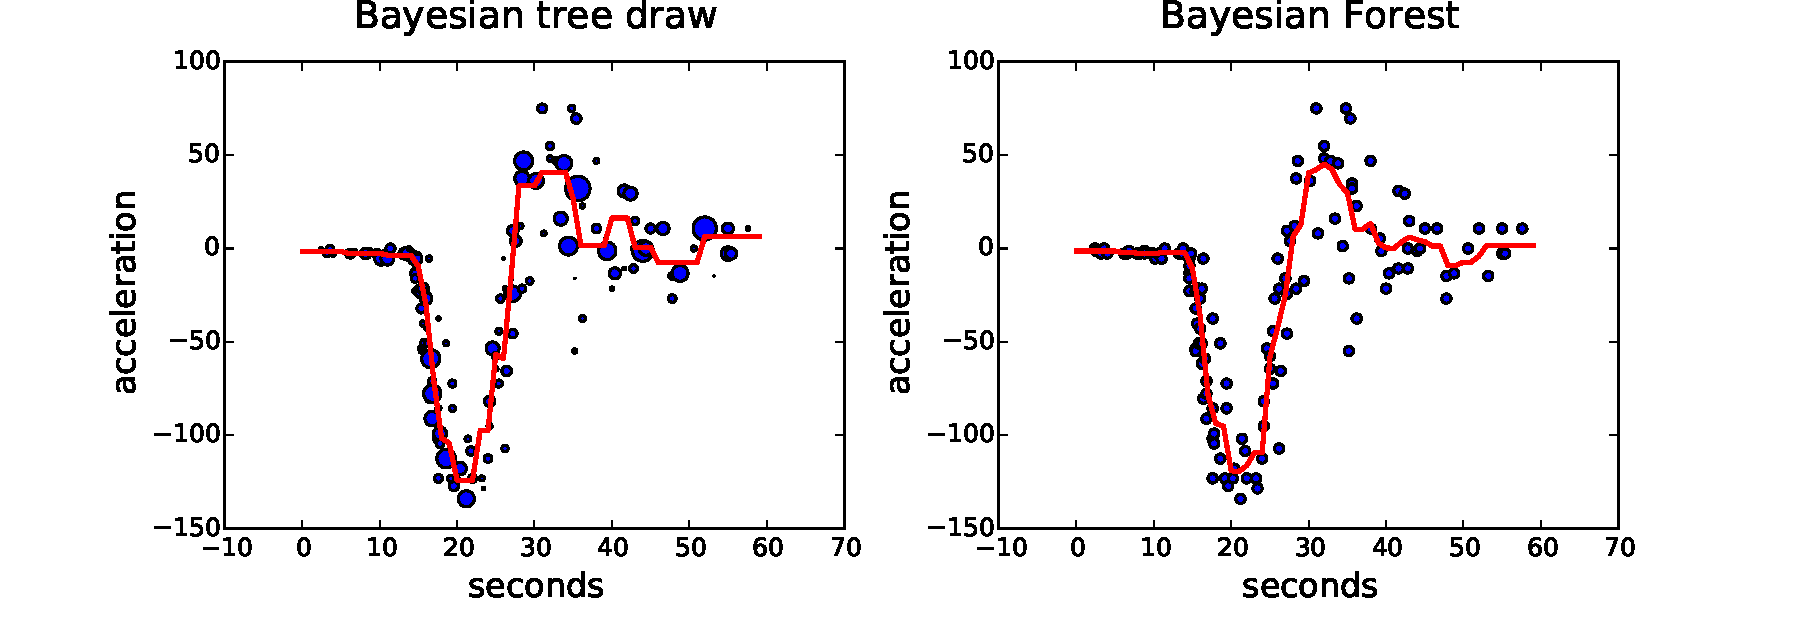
\includegraphics[width=.95\textwidth]{../graphs/mcycle}   

% \end{frame}


\begin{frame}

{\bf Theoretical trunk stability}

\vskip .5cm

Given forests as a posterior, 
we can start talking about {\it variance}.

\vskip .25cm
We are able to derive theoretically that the earliest structure in the tree -- {\theme the trunk} -- should be very stable for large samples.

\vskip .25cm
For the data at a given node, the probability that the optimal split on resampled data matches the true optimal split is
\begin{equation*}
\mathrm{p}\left(\text{split matches sample CART}\right) \gtrsim 1 - \frac{p}{\sqrt{n}} e^{-n},
\end{equation*}
where $p$ is the number of possible split locations and $n$ the number of observations on the current node.  

\vskip .25cm Things are pretty stable, until they aren't: as the tree grows,  node sizes get smaller and chance of a non-optimal split multiplies.

\end{frame}

\begin{frame}

{\bf California Housing Data}


\vskip .5cm

20k observations on median home prices in zip codes.

\vskip .5cm

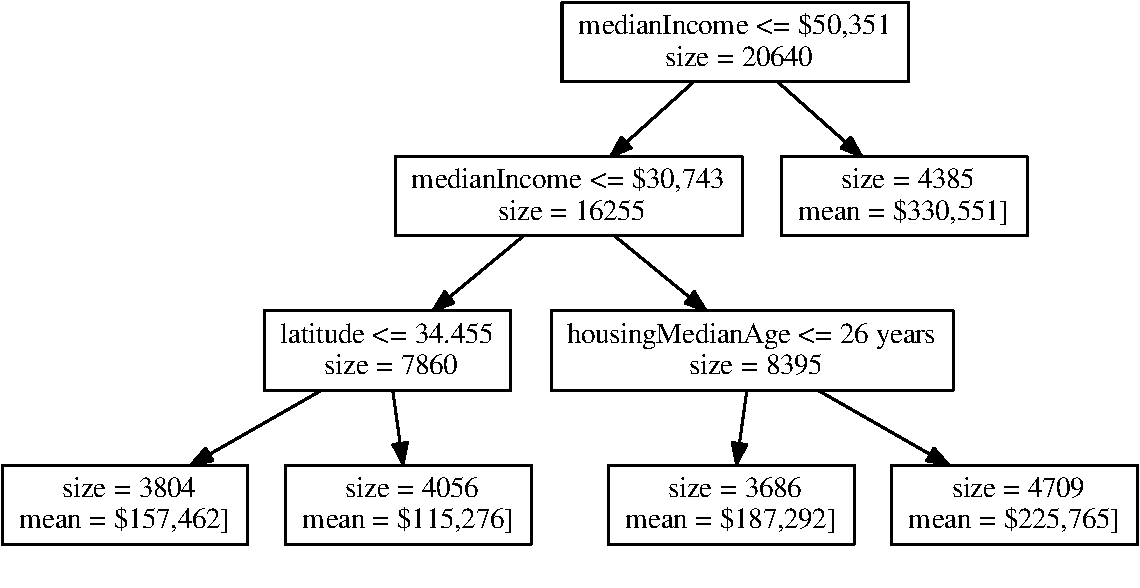
\includegraphics[width=\textwidth]{../graphs/ca_trunk}

\vskip .5cm
\hfill Above is the trunk you get setting min-leaf-size of 3500.

\end{frame}

\begin{frame}

\begin{columns}

\begin{column}{2.15in}
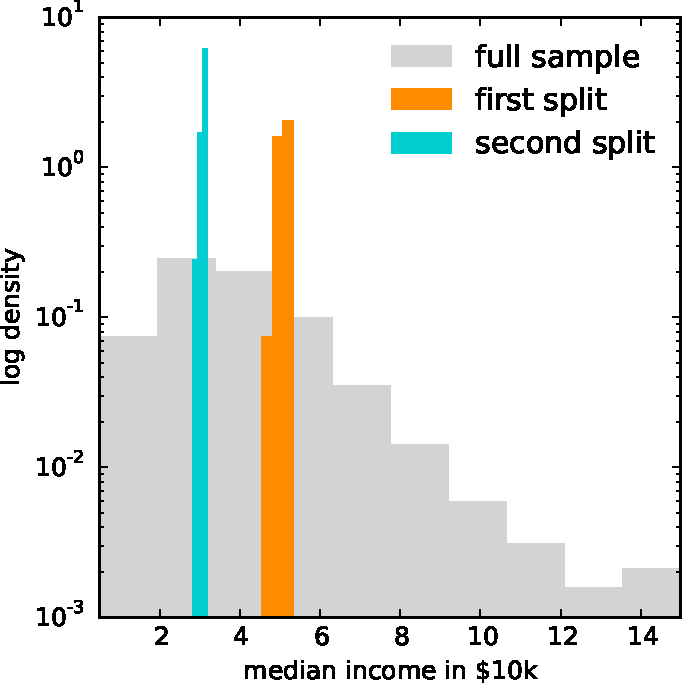
\includegraphics[width=2.5in]{../graphs/ca_splits}
\end{column}

\begin{column}{2in}
\begin{itemize}
\item sample tree occurs 62\% \\of the time.  
\vskip .5cm
\item 90\% of  trees split on income twice, \\and then latitude. 

\vskip .5cm
\item 100\% of trees have 1st 2 splits on median income.  
\end{itemize}
\end{column}

\end{columns}


\vskip 1cm
~~~~Empirically and theoretically: trees are stable, at the trunk.
\vskip -1cm

\end{frame}

\begin{frame}


RFs are expensive when data is too big to fit in memory.

\vskip .2cm
Subsampling forests 
lead to a big drop in performance.

\vskip .2cm
{But wait:}  if the trunks are stable, can we just fit that once and then fit forests at each branch?  {\nv Yes!}

\vskip .5cm
{\bf Empirical Bayesian Forests ({\theme EBF}):}

\vskip .25cm
\begin{itemize}
\item fit a single tree to a shallow {\nv trunk}.  
\item Use this as a mapper to direct full data to each {\nv branch}.  
\item Fit a full  forest on the smaller branch datasets.
\end{itemize}

\vskip .25cm
This is classic Empirical Bayes: fix higher levels in a {\it hierarchical model}, and direct your machinery\texttt{+}data at learning the hard bits.

\end{frame}

\begin{frame}


Since the trunks are all the same for each tree in a full forest,
our EBF looks nearly the same at a fraction of computational cost.

\begin{center}
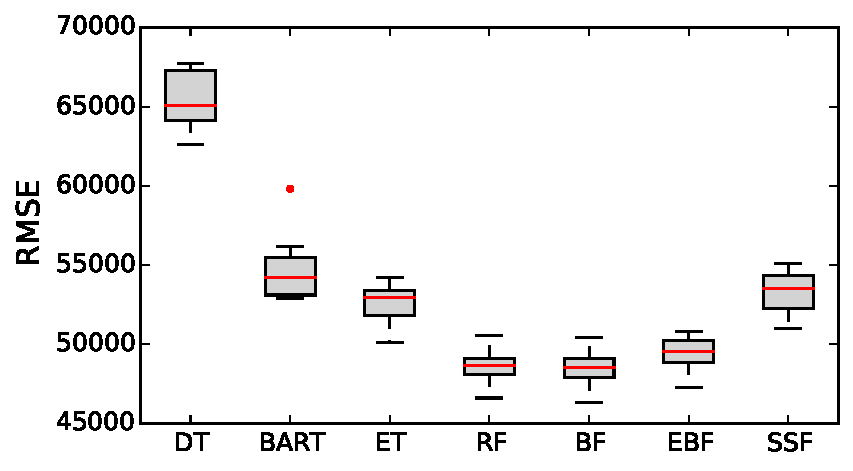
\includegraphics[width=.85\textwidth]{../graphs/ca_rmse}
\end{center}

Here EBF and BF give nearly the same results.  {\it SSF does not.}


\end{frame}


\begin{frame}

{\bf EBFs work all over the place}

\vskip .5cm
\begin{minipage}{0.5\linewidth}
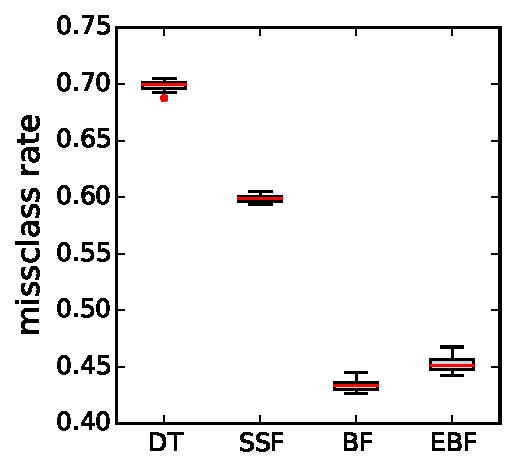
\includegraphics[width=\textwidth]{../graphs/beer}
\end{minipage}
~~
\begin{minipage}{0.4\linewidth}
{\footnotesize
\begin{tabular}{c c | l}
$\overline{\text{MCR}}$  & \% WTB & \\
\cline{1-2}\rule{0pt}{3ex} 
0.4341 &  0.0 & BF \\
0.4531 &  4.4 & EBF \\
0.5989 & 38.0 & SSF \\
0.6979 & 60.8 & DT \\
\end{tabular}}
\end{minipage}

\vskip .5cm
\hfill Predicting beer choice from demographics

\end{frame}

\begin{frame}

{\bf EBFs work all over the place}

\vskip .5cm
\begin{minipage}{0.5\linewidth}
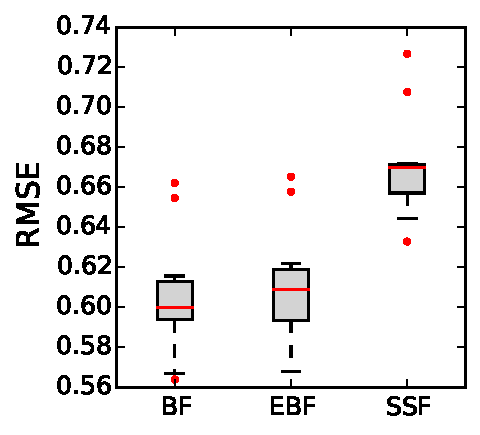
\includegraphics[width=\textwidth]{../graphs/wine}
\end{minipage}
~~
\begin{minipage}{0.4\linewidth}
{\footnotesize
\begin{tabular}{c c | l}
$\overline{\text{RMSE}}$  & \% WTB & \\
\cline{1-2}\rule{0pt}{3ex} 
0.5905 &  0.0 & BF \\
0.5953 &  0.8 & EBF \\
0.6607 & 11.9 & SSF \\
0.7648 & 29.5 & DT \\
\end{tabular}}
\end{minipage}

\vskip .5cm
\hfill or wine rating from chemical profile

\end{frame}

\begin{frame}

{\bf Choosing the trunk depth}


\vskip .5cm
Distributed computing perspective: {\theme fix only as deep as you must!}

\vskip .1cm
How big is each machine? Make that your branch size.

\vskip .75cm
{\small
\begin{tabular}{c | c c c | c c c | c c c}
& \multicolumn{3}{l|}{CA housing} & \multicolumn{3}{l|}{Wine} &\multicolumn{3}{l}{Beer} \\
\cline{2-10} \rule{0pt}{3ex} 
\!\!\!\!\!\!{\it Min Leaf Size in $10^3$} & 6 & 3 & 1.5 & 2  & 1 & 0.5 & 20 & 10 & 5\\
\!\!\!\!\!\!{\it \% Worse Than Best} & \!1.6 & \!2.4 & \!4.3 & \!0.3 & \!0.8 & \!2.2 & \!1.0 & \!4.4 & \!7.6 
\end{tabular}}

\vskip .5cm
Still, open questions.  e.g., more trees vs shallower trunk?

\vskip .25cm
A key point: we {\theme do not} think that EBFs are better than forests fit to all the data.  But EBFs allow you to fit to {\nv much more data} in less time without hurting performance too much.


\vskip .25cm
{\nv Big Data axiom}: more data beats fancy model.

\end{frame}

\begin{frame}


{\bf \theme EBFs at EBay: \bk predicting Bad Buyer Experiences}

\vskip .5cm
A BBE could be receiving something that is `significantly not as described',
or shipping delays, or any of many other problems.

\vskip .5cm
The models are updated frequently, and  information\\ about $\mathrm{p}(\text{BBE})$
is an input to search rankings  and more.

\vskip .2cm The best thing to improve predictions is more data.  \\With millions of daily transactions, there's little limit on data.

\end{frame}

\begin{frame}

{\bf EBFs at EBay}

\vskip .5cm
Full random forest runs take too long on full data \\(even using distributed tree algorithms).

\vskip .5cm
Subsampling led to a noticeable and big drop in performance.

\vskip .5cm
So: EBFs!
\begin{itemize}
\item trunk can be fit in distribution using Spark \texttt{MLLib}.
\item this trunk  acts as a sorting function to map observations \\to 
separate locations corresponding to each branch.
\item Forests are then fit on a machine for each branch.  
\end{itemize}

\end{frame}

\begin{frame}

{\bf EBFs at EBay}

\vskip .5cm

On 12 million transactions,  EBF with 32 branches yields a\\ 1.3\% drop in misclassification over the SSF alternatives.  

\vskip .5cm
This amounts to more than 20,000 extra detected \\BBE occurrences over this short time window.

\vskip .5cm 
Putting it into production requires some careful engineering, \\but this really is {\it a very simple algorithm}.  

\vskip .5cm
If you already fit RFs and are hitting time/space constraints,\\ then an EBF is lots of gain for little pain.

\end{frame}

\begin{frame}

{\theme\bf  The key to big data} 

\vskip .5cm Use plug-in estimates for the stuff that is easy to measure.

\vskip .15cm Partition conditional on these plug-ins.

\vskip .15cm   Direct the full data towards the stuff that is tough to learn.

\vskip 1.5cm
\begin{center}
\Huge
Thanks!
\end{center}

\end{frame}

\end{document}






























